\chapter{Configuration space}

A robot from a mechanical point of view can be seen as a system of $N$ rigid bodies that move in a workspace $W = \mathbb{R} ^2$ or $W = \mathbb{R} ^3$.
The workspace $W$ is the physical space in which the robot operates and can move, it's essentially the geometric space in which the robot operates and can move.
If the workspace is $\mathbb{R} ^2$, the robot is called planar, if the workspace is $\mathbb{R} ^2$ the robot is called spatial.
This definition of a robot is broad enough to allow a group of robots to be defined as a robot.

\begin{definition}
    A configuration $\bm{q}$ is the minimal set of values that fully describe the position and orientation (pose) of the robot (of every point of the robot) at a given time in the workspace.
    $$
        \bm{q} = \begin{bmatrix}
            q_1    \\
            \vdots \\
            q_n
        \end{bmatrix}
    $$
\end{definition}




The components $q_i, \ i =1\dots n$ of a configuration are called generalized components.
The name generalized comes from the fact that the coordinates aren't limited to express only rotations or translations, in fact they can represent any type of motion.
These coordinates generalize the description of the robot’s motion, meaning they adapt to any kind of mechanical system, whether it’s a simple 1D slider or a complex multi-jointed arm in 3D space.

\begin{warningbox}[Warning]
    The special orthonormal group $SO(3)$ describes the orientation of a body using a $3 \times 3$ rotation matrix. Although straightforward, this method is not minimal, as the matrix has 9 elements, with only 3 being independent due to orthonormality constraints, leading to redundancy.

    Euler angles offer a minimal alternative by using 3 parameters (roll, pitch, yaw) to represent the 3 degrees of freedom. However, they suffer from gimbal lock, a singularity where two rotational axes align, causing the loss of one degree of freedom.

    Quaternions, a four-dimensional extension of complex numbers, avoid gimbal lock and efficiently represent rotations. However, they are not minimal either, requiring 4 parameters and a normalization constraint, which introduces redundancy.

    While quaternions are more robust, Euler angles may still be preferred for their minimality, despite the risk of gimbal lock, due to their simpler and more compact representation.
\end{warningbox}

\begin{definition}
    A configuration space $\mathbf{C}$ as the set containing all valid configurations.

    $$
        \mathbf{C}  \{\bm{q} \in \mathbb{R} | \bm{q} \ \text{is a valid configuration of the robot}\}
    $$
\end{definition}

\begin{example}
    Assume we have a robot with a negligible dimension w.r.t to to the workspace $W = \mathbb{R}^3$
    \begin{center}
        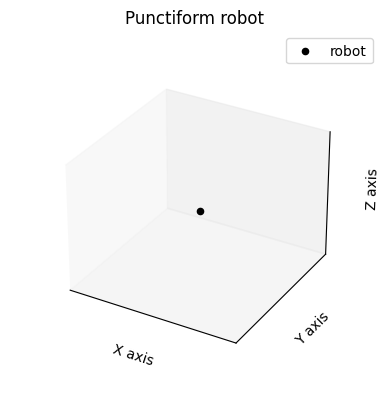
\includegraphics{Configuration space/punctiform_robot.png}
    \end{center}


    In this case the configuration vector is the following
    $$
        \bm{q} = \begin{bmatrix}
            x \\
            y \\
            z
        \end{bmatrix}
    $$
    \begin{tipbox}[Tip]
        In this case $\mathbf{C} = W = \mathbb{R}^3$, this however is not true in general.
    \end{tipbox}
\end{example}

\begin{example}
    Assume we have a circular symmetric robot in the plane, i.e. workspace $W = \mathbb{R}^2$.
    \begin{center}
        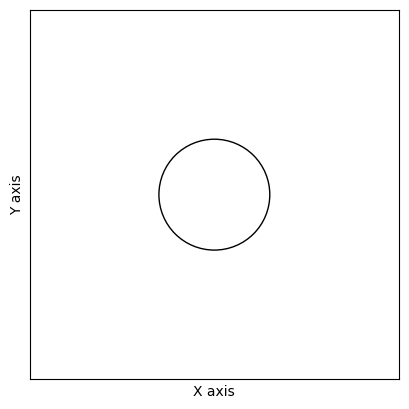
\includegraphics{Configuration space/symmetric_roomba.png}
    \end{center}

    By exploiting it's symmetry, we can express the position of all of it's points w.r.t the center of mass of the robot
    $$
        \bm{q} = \begin{bmatrix}
            x \\
            y
        \end{bmatrix}
    $$
\end{example}

\begin{example}
    Assume we have a circular symmetric robot in the plane, i.e. workspace $W = \mathbb{R}^2$. Now assume that it has a tick on it.

    Now assume this two configurations:

    \begin{center}
        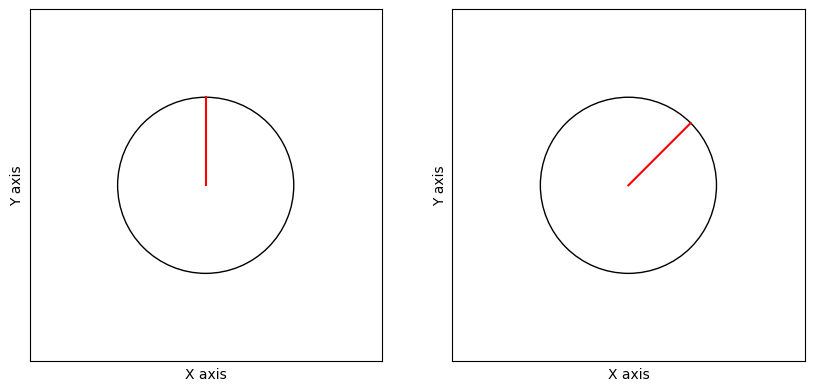
\includegraphics[width=15cm]{Configuration space/asymmetric_roomba.png}
    \end{center}

    If we where to use the previous configuration space we could not distinguish between this two configurations, because while previosly we didn't need to add rotational information, now it's required, thus the generalized vector is:

    $$
        \bm{q} = \begin{bmatrix}
            x \\
            y \\
            \theta
        \end{bmatrix}
    $$

    In which $\theta$ is for example a rotation around the $x$-axis.

    \begin{tipbox}[Tip]
        In this case $\mathbf{C} = \mathbb{R}^2 \times SO(2)$.
    \end{tipbox}

    \begin{warningbox}[Warning]
        While the $SO(3)$ group is redundant, the $SO(3)$  is not, which means that $SO(2)$ is minimal and correctly used.
    \end{warningbox}

    Now, we can represent, for example a positive movement along the $x$ axis as

    \begin{center}
        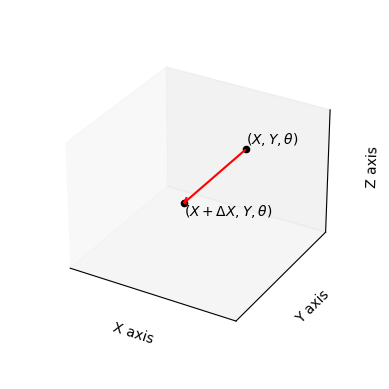
\includegraphics{Configuration space/naive_asymmetric_roomba_configuration_space.png}
    \end{center}

    This is actually \textbf{not} a good representation of the configuration space, however it is convenient because it let's us compress our robot from a volume into a point.
    The need of the configuration space is infact given by the abstraction of the robots geometry.
\end{example}

\begin{example}
    Assume you have a planar manipulator with $N$ joints.

    \begin{center}
        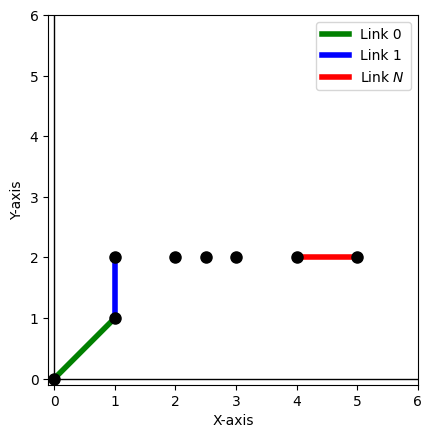
\includegraphics{Configuration space/multi_joint.png}
    \end{center}

    We could describe the configuration of this manupulator by taking as a position the baricenter of each link and thei inclination of each joint, this results in $3N$ parameters.
    This configuration would be great, however it is not minimal.
    A problem, is that assumes that there is no relationship between the links, however we know that the joint pose a constraint which make them dependant.
    Since each joint introduces 2 constraints, the number of free parameters is $3N-2N = N$.

    We can describe the $N$ parameters as

    \begin{center}
        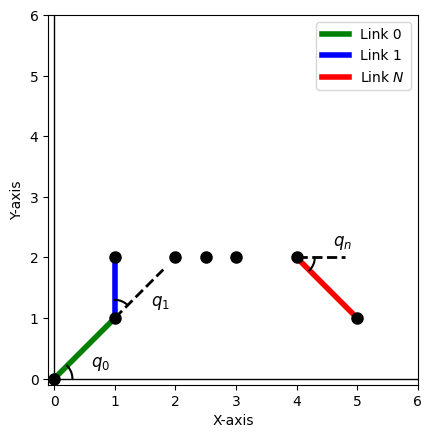
\includegraphics{Configuration space/multi_join_configuration.png}
    \end{center}

    And thus our configuration $\bm{q}$, is just:

    $$
        \bm{q} = \begin{pmatrix}
            q_0    \\
            \vdots \\
            q_n
        \end{pmatrix}
    $$

    While the configuration space is $\mathbf{C} = SO(2)^N$.

    Now, if we assume we have a spatial manipulator, we have $6N$ parameters, of which $3N$ describe the position and $3N$ describe the rotation.
    For everything we said until now, this representation is not minimal, and due to the presence of joints there are $5N$ constraints, which means that we can treat the spatial manipulator as a planar manipulator.
\end{example}


\begin{definition}
    Topology is the study of the fundamental structure and properties of spaces that remain the same even when those spaces are continuously deformed. Topology ignores exact distances or angles and focuses instead on properties like connectedness or the number of holes in a space.
\end{definition}

In robotics, topology becomes crucial when we deal with the robot’s configuration space
The topology of C-space helps us understand whether the robot can smoothly move from one configuration to another without colliding with obstacles. It tells us about the overall shape and connectedness of C-space. Understanding the topology helps in tasks like: motion planning and obstacle avoidance.

Euclidean space is the regular, flat space we’re used to, where distances, angles, and straight lines behave as expected. However, C-space is generally not Euclidean because it doesn't behave like a flat, regular space, in fact it can assume values in $SO(2)$, which is not closed under the sum. In non-Euclidean spaces, distances and paths behave differently.

\begin{example}
    Assume you have a manipulator with two links

    \begin{center}
        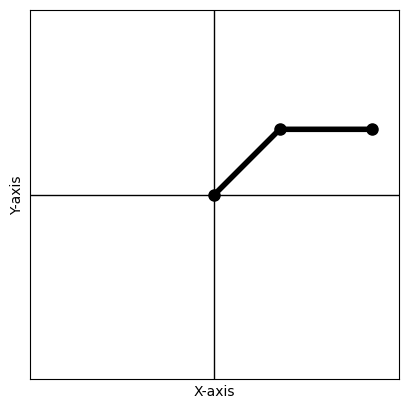
\includegraphics{Configuration space/2R_manipulator.png}
    \end{center}

    Here we have:

    $$
        \bm{q} = \begin{pmatrix}
            q_1 \\
            q2
        \end{pmatrix} \ , \ \mathbf{C} = SO(2) \times SO(2)
    $$

    Now a naive representation of the configuration space would be:

    \begin{center}
        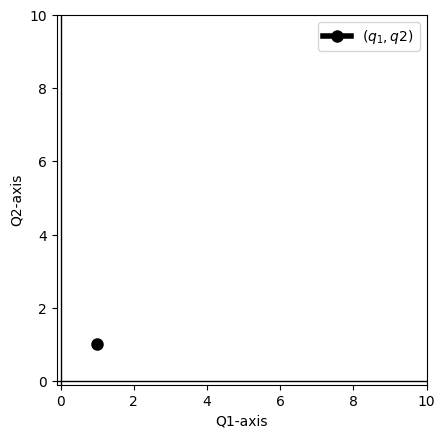
\includegraphics{Configuration space/naive_2R_configuration.png}
    \end{center}

    The first thing, that we notice is that this configuration space is not injective.
    Assume for example that we make a full rotation, around the first axis, the robot will return to the same position, but the configuration will be different:

    \begin{center}
        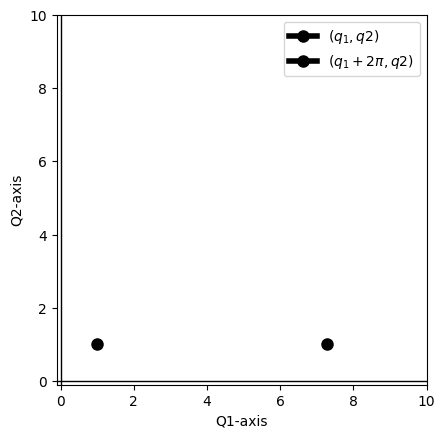
\includegraphics{Configuration space/naive_2R_configuration_non_injectivity.png}
    \end{center}

    In general in fact there will be an infinite values of configurations that in the configuration space describe the same configuration in the working space.

    Now, to solve this we can limit the admissibile values that both $q_1$ and $q_2$ can assume, such that $q_1, \ q_2 \ \in [0,2\pi)$

    \begin{center}
        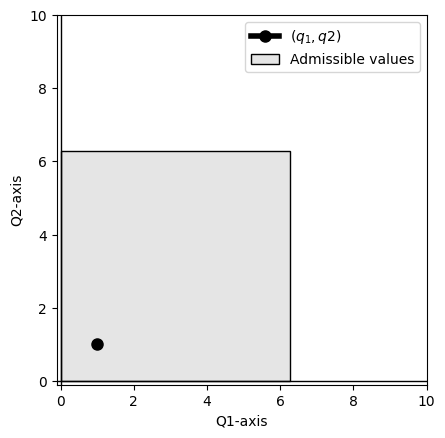
\includegraphics{Configuration space/naive_2R_configuration_injectivity.png}
    \end{center}

    Now, the injectivity problem is solved, however a new problem appears:
    Assume you have two different configurations $q_A = (\epsilon,\pi)$ and $q_B = (2\pi-\epsilon,\pi)$

    \begin{center}
        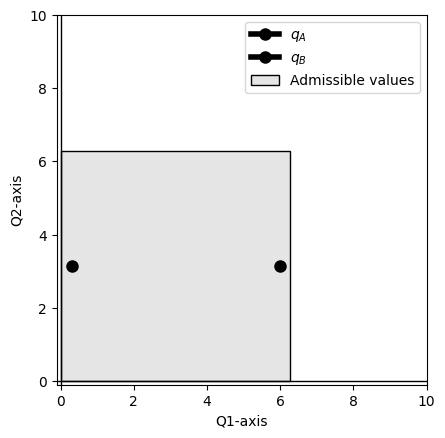
\includegraphics{Configuration space/naive_2R_configuration_distance.png}
    \end{center}

    In the configuration space they seem to be distant, however in the workspace, they appear to be very similar, and thus the distance should be low:

    \begin{center}
        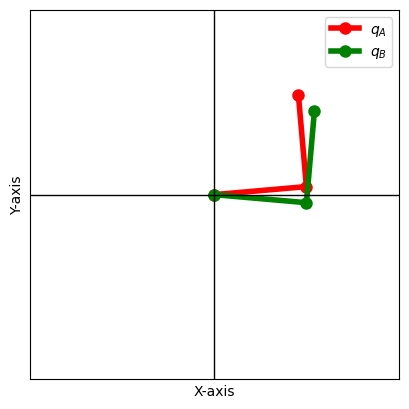
\includegraphics{Configuration space/naive_2R_workspace_distance.png}
    \end{center}

    The problem is, as previously mentioned, that the configuration space is in general not Euclidean.

    We can solve by transforming the admissible zone for the configuration values from a rectangle into a torus

    \begin{center}
        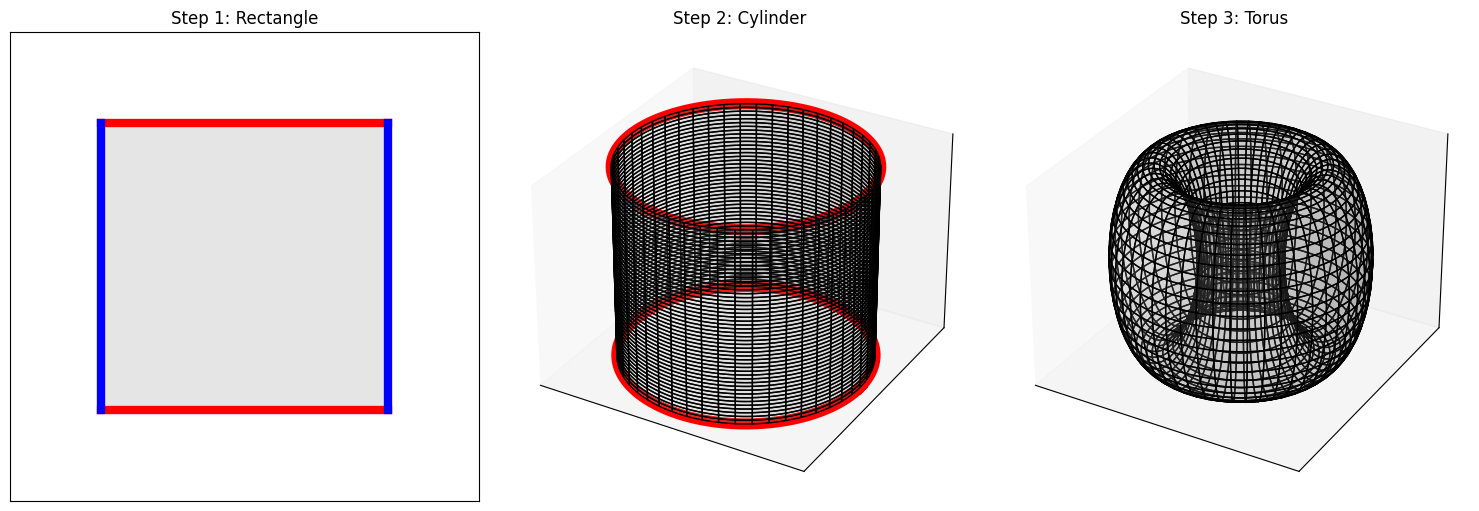
\includegraphics[width=16cm]{Configuration space/rect_to_torus.png}
    \end{center}

    The toroidal configuration space naturally handles the wrap-around behaviors, solving the distance problem.
    A torus is a manifold, which means that locally behaves like the Euclidean space.
    A practical example is the earth, is sperical but locally seems flat.
\end{example}

In general the the configuration space $\mathbf{C}$ is a manifold and only locally presents a Euclidean structure.

We want however, to be able to express the notion of distance, because it reflects some information about similarity of configurations.

\begin{definition}
    A distance $d$ is a valid mathematical function if it has this properties:
    \begin{itemize}
        \item $d(q_a,q_b) \geq 0$
        \item  $d(q_a,q_b) = 0$ iff $q_a = q_b$
        \item $d(q_a,q_b) = d(q_b,q_a)$
        \item $d(q_a,q_b) \leq d(q_a,q_c) + d(q_c,q_b)$
    \end{itemize}
\end{definition}

\begin{warningbox}[Warning]
    Why would we need to define a distance and not just use the euclidean distance ?

    When we talk about Euclidean distance between two points, we're referring to the straight-line (or shortest possible) distance between those points in 3D space.
    Imagine we have a configuration space which has the following form:

    \begin{center}
        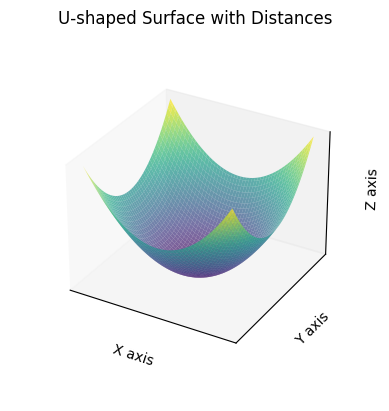
\includegraphics{Configuration space/surface.png}
    \end{center}

    Now assume that we have two configurations $q_a$ and $q_b$, a practical way to see why the euclidean distance is not a good distance is by visualizing.

    \begin{center}
        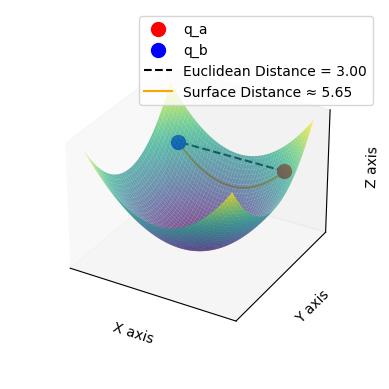
\includegraphics{Configuration space/distance_on_a_manifold.png}
    \end{center}

    The euclidean distance is calculated without accounting for the underlying structure of the configuration space itself.
    While the Euclidean distance may suggest that the configurations are relatively similar due to their proximity in 3D space, it doesn't fully capture the reality of the system's constraints or the manifold the system exists on.

    A more accurate measure of distance within configuration space is the geodesic, which is the shortest path along the curved surface connecting $q_a$ and $q_b$. In this case the geodesic distance indicates that the two configurations are actually quite dissimilar when considering the actual path the system would need to take to move between them.



\end{warningbox}

While geodesics provide a more reliable representation of distance in configuration space, they are generally more difficult to compute, especially in higher-dimensional spaces or when the surface is complex.
In general the displacement metric is used instead.

\begin{definition}
    Given a point $p$ on the robot and $p(\bm{q})$ the position of point $p$ in configuration $\bm{q}$, the displacement metric is the following distance:

    $$
        d(q_a,q_b) = \underset{p \in robot}{max} ||p(a_a) - p(q_b)||
    $$
\end{definition}

The displacement metric is essentially the maximum distance of all the points between two different configurations.

\begin{tipbox}
    We have moved the definition of distance from the configuration space to the workspace, which is an euclidean space and the euclidean distance is well defined.
\end{tipbox}

A good way to understand the displacement metric is to visualize it

\begin{center}
    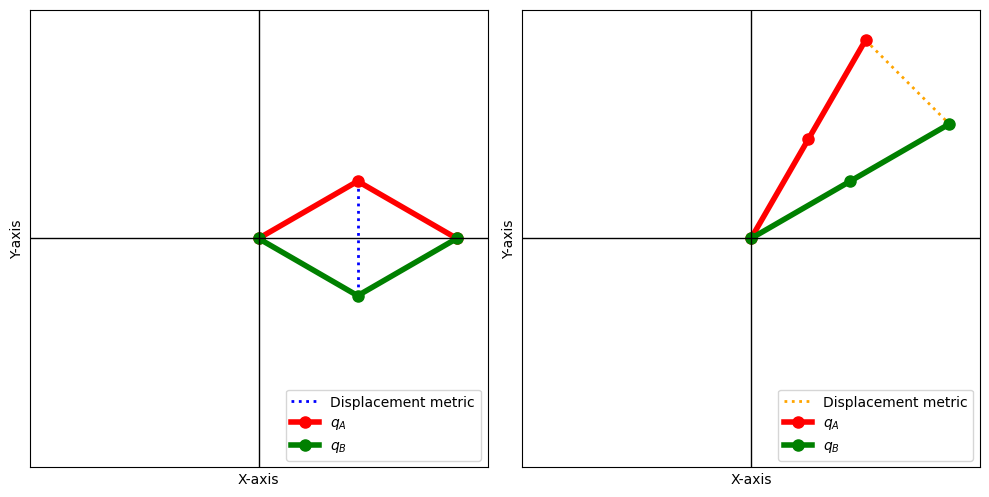
\includegraphics[width = 15cm]{Configuration space/ok_displacement_metric.png}
\end{center}

An obvious problem with this approach is the fact that we want to determine the maximum in a set of infinite pairs, which means that when implementing it in a software we should need to do an infinite number of computations.

To solve this issue we can focus on just $N$ points called central points, predefined and which reduces the infinity of points to a finite number.

Another problem is the fact that the $max$ is not differentiable, and thus we cannot optimize, it, so instead, to solve both problems we give a new mathematical formulation for the displacement metric:

$$
    d'(a_a,q_b) = \sum_{i=1}^N || p_i(q_a) - p_i(q_b)||
$$

\begin{warningbox}
    By leveraging the fact that locally the manifold behaves like an euclidean space we can use the euclidean distance if the points are known to be close.
\end{warningbox}